\documentclass[11pt,twoside,a4paper]{article}
% http://www-h.eng.cam.ac.uk/help/tpl/textprocessing/latex_maths+pix/node6.html symboles de math
% http://fr.wikibooks.org/wiki/Programmation_LaTeX Programmation latex (wikibook)
%=========================== En-Tete =================================
%--- Insertion de paquetages (optionnel) ---
\usepackage[french]{babel}   % pour dire que le texte est en fran{\'e}ais
\usepackage{a4}	             % pour la taille   
\usepackage[T1]{fontenc}     % pour les font postscript
\usepackage{epsfig}          % pour gerer les images
%\usepackage{psfig}
\usepackage{float}           % pour le placement des figures
\usepackage{verbatim}

\usepackage{longtable} % pour les tableaux de plusieurs pages

\usepackage[table]{xcolor} % couleur de fond des cellules de tableaux

\usepackage{lastpage}

\usepackage{multicol} % pour {\'e}crire dans certaines zones en colonnes : \begin{multicols}{nb colonnes}...\end{multicols} 

% \usepackage[top=1.5cm, bottom=1.5cm, left=1.5cm, right=1.5cm]{geometry}
% gauche, haut, droite, bas, entete, ente2txt, pied, txt2pied
\usepackage{vmargin}
\setmarginsrb{1.00cm}{1.00cm}{1.00cm}{1.00cm}{15pt}{3pt}{15pt}{3pt}

\usepackage{lscape} % changement orientation page
%\usepackage{frbib} % enlever pour obtenir references en anglais
% --- style de page (pour les en-tete) ---
\pagestyle{empty}

% % % en-tete et pieds de page configurables : fancyhdr.sty

% http://www.trustonme.net/didactels/250.html

% http://ww3.ac-poitiers.fr/math/tex/pratique/entete/entete.htm
% http://www.ctan.org/tex-archive/macros/latex/contrib/fancyhdr/fancyhdr.pdf
% \usepackage{fancyhdr}
% \pagestyle{fancy}
% % \newcommand{\chaptermark}[1]{\markboth{#1}{}}
% % \newcommand{\sectionmark}[1]{\markright{\thesection\ #1}}
% \fancyhf{}
% \fancyhead[LE,RO]{\bfseries\thepage}
% \fancyhead[LO]{\bfseries\rightmark}
% \fancyhead[RE]{\bfseries\leftmark}
% \fancyfoot[LE]{\thepage /\pageref{LastPage} \hfill
	% TITLE
% \hfill 
\includegraphics[width=0.5cm]{img/logo_glider.png} }
% \fancyfoot[RO]{
\includegraphics[width=0.5cm]{img/logo_glider.png} \hfill
	% TITLE
% \hfill \thepage /\pageref{LastPage}}
% \renewcommand{\headrulewidth}{0.5pt}
% \renewcommand{\footrulewidth}{0.5pt}
% \addtolength{\headheight}{0.5pt}
% \fancypagestyle{plain}{
	% \fancyhead{}
	% \renewcommand{\headrulewidth}{0pt}
% }

%--- Definitions de nouvelles commandes ---
\newcommand{\N}{\mathbb{N}} % les entiers naturels

%============================= Corps =================================

\begin{document}

\setlength\parindent{0pt} % \noindent for all document

\texttt{http://passeurdesciences.blog.lemonde.fr/2012/09/12/quelle-probabilite-pour-un-nouveau-11-septembre/} %% ~\\

\textbf{\LARGE Quelle probabilit{\'e} pour un nouveau 11-Septembre ?}%% ~\\

\textcolor{gray}{ \textbf{\large 12 septembre 2012, par Pierre Barth{\'e}l{\'e}my} }

\begin{multicols}{2}
	\footnotesize

	\begin{center} 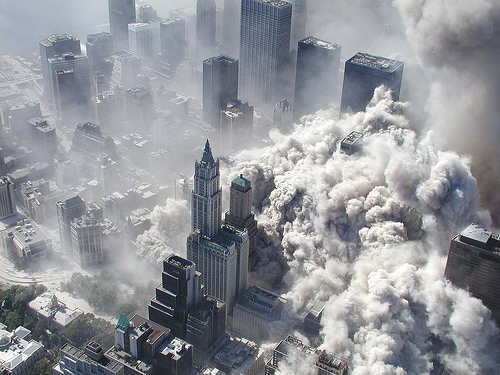
\includegraphics[width=0.47\textwidth]{WTC.jpg} \end{center} 
	
	\textbf{Les actes terroristes} peuvent se mettre en {\'e}quation. C'est du moins l'avis d'Aaron Clauset~\footnotemark. Depuis quelques ann{\'e}es, ce chercheur de l'universit{\'e} du Colorado analyse une immense base de donn{\'e}es qui, courant sur la p{\'e}riode 1968-2007, compile 13 274 attentats meurtriers de par le monde. Pour ce chercheur passionn{\'e} par les syst{\`e}mes complexes, qui traque les structures math{\'e}matiques cach{\'e}es dans les conflits humains, la machine infernale du terrorisme se traduit en formules, en mod{\`e}les et en points distribu{\'e}s le long de courbes. En 2007, dans un article publi{\'e} par The Journal of Conflict Resolution~\footnotemark, Aaron Clauset, {\'e}paul{\'e} par deux coll{\`e}gues, Maxwell Young et Kristian Skrede Gleditsch, a montr{\'e} que les actions terroristes r{\'e}pertori{\'e}es dans cette base de donn{\'e}es suivent une loi de puissance : un attentat est d'autant moins fr{\'e}quent qu'il fait beaucoup de victimes. Cela semble {\'e}vident mais encore fallait-il le v{\'e}rifier. Le m{\^e}me genre de loi est retrouv{\'e} et exploit{\'e} par des chercheurs travaillant sur les s{\'e}ismes, les feux de for{\^e}ts, les avalanches ou... krachs boursiers. On peut donc a priori, dans un contexte donn{\'e}, {\'e}valuer la probabilit{\'e} pour qu'un ou des attentats plus ou moins sanglants se produisent. ~\\
		\footnotetext{\texttt{http://tuvalu.santafe.edu/\textasciitilde aaronc/}}
		\footnotetext{\texttt{http://jcr.sagepub.com/content/51/1/58.abstract}}
	
	\textbf{Toute la difficult{\'e} de l'exercice}, qui int{\'e}resse de pr{\`e}s politiques et militaires outre-Atlantique~\footnote{\texttt{http://www.psmag.com/culture/the-physics-of-terror-25955/}}, c'est de savoir si les {\'e}v{\'e}nements extr{\^e}mes entrent ou non dans ce cadre. En bref, de savoir si les attentats du 11 septembre 2001, qui ont fait pr{\`e}s de 3 000 morts aux Etats-Unis, s'inscrivent dans la courbe, s'il est possible d'estimer r{\'e}trospectivement leur probabilit{\'e} en fonction du contexte de l'{\'e}poque ou bien s'ils constituent ce que les statisticiens appellent des "donn{\'e}es aberrantes", des {\'e}v{\'e}nements compl{\`e}tement improbables. Le 11-Septembre, par son caract{\`e}re exceptionnel, puisqu'il a {\'e}t{\'e} cinq fois plus meurtrier que son "dauphin" sur le podium de l'horreur (l'attentat du 14 ao{\^u}t 2007 dans la ville irakienne de Sinjar : 572 morts), est un bon test pour les mod{\`e}les. ~\\
	
	\textbf{Dans un article mis en ligne} le 1er septembre sur le site de pr{\'e}-publications scientifiques arXiv~\footnote{\texttt{http://arxiv.org/abs/1209.0089}}, Aaron Clauset et Ryan Woodard s'attaquent {\`a} la question gr{\^a}ce {\`a} un algorithme de leur composition. Celui-ci s'av{\`e}re {\'e}tonnamment robuste : il fonctionne correctement sur les quatre d{\'e}cennies couvertes par les statistiques, alors m{\^e}me qu'au cours de cette longue p{\'e}riode, le terrorisme a chang{\'e} de visage et de mode d'action, notamment avec l'{\'e}mergence et la mont{\'e}e en puissance des attentats-suicides. Pour en revenir au 11-Septembre, les deux chercheurs ont fait tourner quatre mod{\`e}les diff{\'e}rents. Le r{\'e}sultat fait un peu froid dans le dos. Suivant les mod{\`e}les, il y avait, sur les quatre derni{\`e}res d{\'e}cennies, entre 11 et 35 \% de risques qu'un tel {\'e}v{\'e}nement se produise. Une valeur "inconfortablement {\'e}lev{\'e}e", notent les auteurs. M{\^e}me dans le "meilleur" des cas, la probabilit{\'e} est loin de z{\'e}ro et, pour ces chercheurs, le 11-Septembre ne constitue en aucun cas une "donn{\'e}e aberrante". ~\\
	
	\textbf{Forc{\'e}ment, dans ce genre d'{\'e}tudes}, se pose toujours la question du futur. Quelle est la probabilit{\'e} pour que l'on assiste, au cours des dix prochaines ann{\'e}es, {\`a} un attentat d'une telle ampleur, voire plus grave ? Aaron Clauset et Ryan Woodard ont test{\'e} trois sc{\'e}narios diff{\'e}rents. Le premier, optimiste, parie sur un apaisement en Irak~\footnote{\texttt{http://www.lemonde.fr/proche-orient/article/2012/09/10/pres-de-100-morts-dans-une-vingtaine-d-attentats-en-irak\_1757975\_3218.html}} et en Afghanistan, o{\`u} l'on d{\'e}nombre beaucoup d'attentats, et sur un nombre annuel d'actes terroristes limit{\'e} {\`a} 400 (moyenne de la p{\'e}riode 1998-2002). Le deuxi{\`e}me table sur un nombre d'attentats se maintenant au niveau de 2007, soit 2 000 par an. Le troisi{\`e}me, tr{\`e}s pessimiste, voit ce nombre monter en fl{\`e}che et atteindre les 10 000. Dans le premier cas, le risque d'assister {\`a} un {\'e}quivalent du 11-Septembre est relativement bas, dans une fourchette de 4 {\`a} 12 \%. Dans le deuxi{\`e}me sc{\'e}nario, le risque est compris entre 19 et 46 \%, soit davantage que pour le 11-Septembre. Dans le troisi{\`e}me et dernier cas de figure, celui d'une recrudescence mondiale du terrorisme, le risque se situe entre 64 et 94 \% : plus fr{\'e}quentes sont les attaques terroristes sur la plan{\`e}te, plus grande est la probabilit{\'e} de voir survenir au moins un {\'e}v{\'e}nement de grande ampleur. ~\\
	
	\textbf{Les deux auteurs ont conscience} que leurs fourchettes sont larges et ils donnent des pistes pour les affiner : introduire des {\'e}l{\'e}ments de contexte g{\'e}opolitique, des donn{\'e}es sur l'acc{\`e}s aux technologies, sur la d{\'e}mographie, sur la lutte contre le terrorisme, etc. Aaron Clauset et Ryan Woodard reconnaissent aussi que leur algorithme ne dit pas o{\`u} risquent de se produire les plus gros attentats mais ils envisagent de combler -- du moins en partie -- cette lacune en incorporant une grille g{\'e}ographique avec un maillage de plus en plus fin au fil du temps, suivant en cela ce que font les sismologues. ~\\
	
	\textbf{Reste un ultime probl{\`e}me}, qui ne figure qu'en creux dans l'{\'e}tude. Les courbes pr{\'e}sent{\'e}es ne s'arr{\^e}tent pas qu'{\`a} des {\'e}v{\'e}nements faisant 3 000 victimes comme le 11-Septembre. Elles se poursuivent. Sur mon pr{\'e}c{\'e}dent blog~\footnote{\texttt{http://blog.slate.fr/globule-et-telescope/2011/01/03/le-terrorisme-cest-mathematique/}}, j'avais consacr{\'e} un billet {\`a} cette mise en {\'e}quation du terrorisme et repris une citation extraite d'une interview d'Aaron Clauset o{\`u} il r{\'e}pondait {\`a} la question du pire. Pire que le 11-Septembre, c'est quoi ? A l'{\'e}poque, le chercheur am{\'e}ricain r{\'e}pondait ainsi : ``\emph{Le danger vient essentiellement du nucl{\'e}aire. Il est tout {\`a} fait dans le domaine du possible que, au cours des 50 prochaines ann{\'e}es, une petite bombe atomique explose quelque part dans le monde lors d'une attaque terroriste. }'' Pour le moment, Aaron Clauset n'a pas encore donn{\'e} le chiffre de probabilit{\'e}. %% ~\\
	
	\begin{flushright}
		\textbf{Pierre Barth{\'e}l{\'e}my} (\texttt{@PasseurSciences~\footnote{\texttt{https://twitter.com/\#\%21/PasseurSciences}}} sur Twitter)
	\end{flushright}
\end{multicols}

\end{document}